\documentclass[tikz,border=0pt]{standalone}
\usepackage{amsmath}
\usepackage{tikz}
\usetikzlibrary{arrows.meta,calc,patterns,decorations.pathmorphing}
\begin{document}
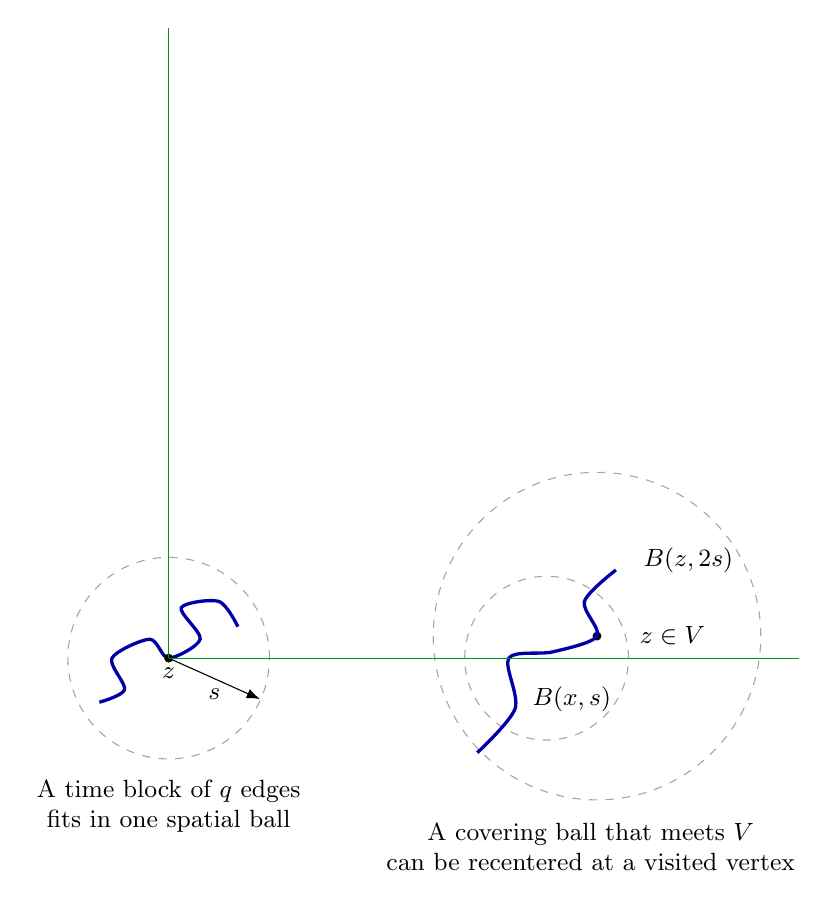
\begin{tikzpicture}[scale=.8,font=\small,>=Latex]
\draw[gray!70,dashed] (0,0) circle (1.6);
\draw[blue!65!black,very thick] plot[smooth] coordinates {(-1.1,-.7) (-.7,-.5) (-.9,0) (-.3,.3) (0,0) (.5,.3) (.2,.8) (.8,.9) (1.1,.5)};
\fill (0,0) circle (2pt) node[below] {$z$};
\draw[->] (0,0)--(1.45,-.65) node[midway,below] {$s$};
\node[align=center] at (0,-2.35) {A time block of $q$ edges\\fits in one spatial ball};
\begin{scope}[xshift=6cm]
\draw[gray!70,dashed] (0,0) circle (1.3);
\draw[gray!70,dashed] (.8,.35) circle (2.6);
\fill (.8,.35) circle (2pt) node[right,xshift=12pt] {$z\in V$};
\draw[blue!65!black,very thick] plot[smooth] coordinates {(-1.1,-1.5) (-.5,-.8) (-.6,0) (.1,.1) (.8,.35) (.6,.9) (1.1,1.4)};
\node at (.4,-.65) {$B(x,s)$};
\node at (2.25,1.55) {$B(z,2s)$};
\node[align=center] at (.7,-3) {A covering ball that meets $V$\\can be recentered at a visited vertex};
\end{scope}
\draw[green!60!black,line width=0.4pt] (0,0)--(10,0)(0,0)--(0,10);\end{tikzpicture}
\end{document}
